\chapter{what is blitting}
\label{sec:listing}
\lstset{style=6502Style}

Blitting is the process of writing pixels to the screen. A bltter is a \textit{bit block processor}. When we \textit{blit} an image
to the screen we are copying a specific block of image data from storage to the screen where the user can see it.

This short extract from the routine that looks after the 'High Score' table in Tempest 200 gives you an idea of how easy using the blitter
can be. All we have to do is point at the position in RAM containing our pixel data (in this case the pixels from \icode{beasty7.cry} that
we loaded to \icode{pic5}), tell the blitter the x and y position we want to copy from, the width and height we want to copy, and
the x and y position on the screen we want to copy to.

\begin{lstlisting}[escapechar=\%]
  ; Paint the 'Top Guns' graphic
  move.l #pic5,a0    ; file images/beasty7.cry, our source data.
  move.l #screen3,a1 ; the destination we're copying to.
  move #1,d0         ; x position in pic5
  move #1,d1         ; y position in pic5
  move #223,d2       ; width of block to copy
  move #79,d3        ; height of block to copy 
  move #70,d4        ; x pos of destination
  move #10+8,d5      ; y pos of destination
  jsr CopyBlock
\end{lstlisting}

So in the above we specify a block in the image data from \textit{beasty7.cry} opposite from the top-left corner (x:1, y:1) with a width of 223 pixels and a height of 79
pixels. We then tell it that we want to write this to x position 70 and y position 18 on the screen, in other words somewhere just offset from the top left of the screen. 
This is the piece of the image we are selecting for copying:

\begin{figure}[H]
    \centering
    \begin{adjustbox}{width=5cm,center}
      \frame{
\includegraphics[width=12cm]{src/blitting/topgun.png}}%
    \end{adjustbox}
\caption{The bit of \icode{beasty7.cry} we've selected for copying.}
\end{figure}

If we look more closely at the snippet I extracted above we can wee that We seem to be doing this 'specifying' by moving our values into things called \icode{a0}, \icode{a1}, \icode{d0}, \icode{d1}, and so on. 
These are 'registers'. An old computer such as the Motorola 68K CPU in the Atari Jaguar has only so many fingers and thumbs it can use
for counting, and these are them. \icode{a0}, \icode{a1} and so on are 'address registers'. So if we have the address of a piece of code
or data we want the CPU to use an 'address register' is where we store them. If we have some 'values' on the other hand, i.e. some numbers,
then the 'data registers' \icode{d0,d1} are where we put them. 

As you read on you'll find it's a common pattern in Tempest 2000's source code to load up a bunch of registers with bits and pieces and then
call a function (or 'routine' in assembler parlance) that expects those registers to contain the values it should work with. If this sounds
familiar, and that we are essentially using these registers as parameters to a function, then you are correct: that's exactly what we're
doing. 

The simple operation we're performing here is to copy a portion of the \icode{beasty7.cry} image file to the screen. The \icode{CopyBlock}
routine opposite just needs to know the position and dimensions of the portion we're copying and the position on the screen we want to place
it. To achieve this the snippet of game code on the previous page sets up the registers as follows:

\begin{figure}[H]
  {
    \setlength{\tabcolsep}{3.0pt}
    \setlength\cmidrulewidth{\heavyrulewidth} % Make cmidrule = 
    \begin{adjustbox}{width=10cm,center}

      \begin{tabular}{llll}
        \toprule
        Register & Type & Value & Description\\
        \midrule
        \icode{a0} & Address & \icode{pic5} & Source Screen\\
        \icode{a1} & Address & \icode{screen3} & Destination Screen\\
        \icode{d0} & Data & \icode{1} & X Position in Source Screen\\
        \icode{d1} & Data & \icode{1} & Y Position in Source Screen\\
        \icode{d2} & Data & \icode{223} & Width to Copy\\
        \icode{d3} & Data & \icode{79} & Height to Copy\\
        \icode{d4} & Data & \icode{70} & X Position in Destination Screen to Copy to\\
        \icode{d5} & Data & \icode{18} & Y Position in Destination Screen to Copy to\\
        \bottomrule
      \end{tabular}
    \end{adjustbox}
  }\caption*{Setting up the registers for \icode{CopyBlock}.}
\end{figure}

\clearpage
\begin{lstlisting}[escapechar=\%]
CopyBlock:
;
; Copy from screen at a0 to screen at a1
; d0/d1=origin of sourceblock
; d2/d3=width and height of block to copy
; copy from blitter a1 to a2.
; d4/d5=destination XY
;
; This simple routine will assume both screens are the same width
; Using this blitter is a piece of piss.

  move.l #PITCH1|PIXEL16|WID320|XADDINC,d7
  move.l d7,A1_FLAGS  ;a1 (Source) Gubbins

  move.l #PITCH1|PIXEL16|WID384|XADDPIX|YADD1,d7
  move.l d7,A2_FLAGS  ;a2 (Dest) Gubbins

  move d3,d7
  swap d7
  move d2,d7
  move.l d7,B_COUNT   ;set inner and outer loop counts

  move d1,d7
  swap d7
  move d0,d7
  move.l d7,A1_PIXEL  ;origin of source

  move d5,d7
  swap d7
  move d4,d7
  move.l d7,A2_PIXEL  ;origin of destination

  move.l #0,A1_FPIXEL


  move.l #$0001,A1_INC
  move.l #$0,A1_FINC

  move #1,d7
  swap d7
  move d2,d7
  neg d7
  move.l d7,A1_STEP
  move.l d7,A2_STEP    ;set loop steps

  move.l a0,d7
  move.l d7,A1_BASE
  move.l a1,d7
  move.l d7,A2_BASE    ;set screen window bases

  move.l #SRCEN|UPDA1|UPDA2|DSTA2|LFU_A|LFU_AN,d7
  move.l d7,B_CMD
  bra WaitBlit
\end{lstlisting}

\begin{definition}[claw says\index{claw says}]
\setlength{\intextsep}{0pt}%
\setlength{\columnsep}{3pt}%
\begin{wrapfigure}{l}{0.09\textwidth}

\includegraphics[width=\linewidth]{src/callout/claw.png} 
\end{wrapfigure}
\small
\textcolor{white}{
  The source and destination are described as 'screens' in the Tempest 2000 code. This is a useful way of thinking of our pixel data, which
  although it is just a list of bytes, always represents a screen of a certain height and width. While in practice we are copying a section from an image
  to the screen here, we can think of it as copying from one screen to another - with the destination screen the one being shown to the player.
}
\end{definition}

The mechanics of how the \icode{CopyBlock} routine uses this information to actually copy a segment of our image
to the screen are not obvious to the unintiated. This is because it involves a lot of precise specification of many different
instructions to the Blitter (Bit Block Processor) hardware. The amount of set up involved makes our preparation of the \icode{a0-a1}
and \icode{d0-d5} registers look modest in comparison. There is a quite involved amount of bit-twiddling required to get the Blitter
set up the way we want it. Using this routine may be a 'piece of piss', but writing it was fairly painstaking. For example:

\begin{lstlisting}[escapechar=\%]
  move.l #PITCH1|PIXEL16|WID320|XADDINC,d7
  move.l d7,A1_FLAGS  ;a1 (Source) Gubbins
\end{lstlisting}

Here we are formulating some of the parameters we want the Blitter to use when it copies the pixels from our source. We're combining
the parameters into a single 64-bit value, storing it in the \icode{d7} data register and then writing that to the Blitter's \icode{A1\_FLAGS}
register. This is the register it will read to figure out some of the things we want to do with the copy operation.

\begin{figure}[H]
  {
    \setlength{\tabcolsep}{3.0pt}
    \setlength\cmidrulewidth{\heavyrulewidth} % Make cmidrule = 
    \begin{adjustbox}{width=12cm,center}

      \begin{tabular}{llll}
        \toprule
        Parameter & Bits & Hex & Description\\
        \midrule
        \icode{PITCH1}   & \icode{00000000 00000000 00000000 00000000 } & \icode{00000000} & Pixel data has no gaps\\
        \icode{PIXEL16}  & \icode{00000000 00000000 00000000 00110000 } & \icode{00000020} & Pixel Size 16 bits\\
        \icode{WID320}   & \icode{00000000 00000000 01000010 00000000 } & \icode{00004200} & Screen Width of 320\\
        \icode{XADDINC}  & \icode{00000000 00000011 00000000 00000000 } & \icode{00030000} & Add 1 to X at each pass\\
        \midrule
        \icode{A1\_FLAGS}& \icode{00000000 00000011 01000010 00110000 } & \icode{00034220} & Blitter's A1 Flags Register\\
        \bottomrule
      \end{tabular}
    \end{adjustbox}
  }\caption*{Combining our parameters into the Blitter's A1 Flags Register.}
\end{figure}

There is a lot more of this kind of thing in there and it would definitely be too tedious to itemize each operation here in detail.
But there is at least one other pattern worth pointing out in the routine, exemplified by the following snippet that copies the X (\icode{d0})
and Y (\icode{d1}) positions in \textit{beasty7.cry} that we are telling the blitter to use as its origin for copying:

\begin{lstlisting}[escapechar=\%]
  move d1,d7
  swap d7
  move d0,d7
  move.l d7,A1_PIXEL  ;origin of source
\end{lstlisting}

Here the \icode{A1\_PIXEL} register we're writing to (like all our address and data registers) is 32-bits (or 4 bytes) long. This means it can
contain both our X and Y values which will be at most 2 bytes long each. So to get our \icode{d0} and \icode{d1} values in there we first write
the \icode{d1} value to \icode{d7} giving:

\begin{figure}[H]
  {
    \setlength{\tabcolsep}{3.0pt}
    \setlength\cmidrulewidth{\lightrulewidth} % Make cmidrule = 
    \begin{adjustbox}{width=3cm,center}
      \begin{tikzpicture}
      \def\BACKGROUNDONE{lightgreen}
      \fill[\BACKGROUNDONE] (2,0) rectangle ++ (1,1);
      \fill[\BACKGROUNDONE] (3,0) rectangle ++ (1,1);
        \draw[step=1.0,gray,thin] (0,0) grid (1,1);
        \node[matrix of math nodes,anchor=south west,inner sep=0pt,
        nodes={draw,minimum size=1cm,anchor=center},
        column sep=-\pgflinewidth,row sep=-\pgflinewidth,font=\huge\ttfamily]
        {
          00 & 00  & 00 & 01 \\
        };
      \end{tikzpicture}
    \end{adjustbox}
  }
\end{figure}
\vspace{-0.5cm}
Next, we swap its position:
\begin{figure}[H]
  {
    \setlength{\tabcolsep}{3.0pt}
    \setlength\cmidrulewidth{\lightrulewidth} % Make cmidrule = 
    \begin{adjustbox}{width=3cm,center}
      \begin{tikzpicture}
      \def\BACKGROUNDONE{lightgreen}
      \fill[\BACKGROUNDONE] (0,0) rectangle ++ (1,1);
      \fill[\BACKGROUNDONE] (1,0) rectangle ++ (1,1);
        \draw[step=1.0,gray,thin] (0,0) grid (1,1);
        \node[matrix of math nodes,anchor=south west,inner sep=0pt,
        nodes={draw,minimum size=1cm,anchor=center},
        column sep=-\pgflinewidth,row sep=-\pgflinewidth,font=\huge\ttfamily]
        {
          00 & 01  & 00 & 00 \\
        };
      \end{tikzpicture}
    \end{adjustbox}
  }
\end{figure}
\vspace{-0.5cm}
Now we write \icode{d0} to \icode{d7}: 
\begin{figure}[H]
  {
    \setlength{\tabcolsep}{3.0pt}
    \setlength\cmidrulewidth{\lightrulewidth} % Make cmidrule = 
    \begin{adjustbox}{width=3cm,center}
      \begin{tikzpicture}
      \def\BACKGROUNDONE{lightgreen}
      \def\BACKGROUNDTWO{lightblue}
      \fill[\BACKGROUNDONE] (0,0) rectangle ++ (1,1);
      \fill[\BACKGROUNDONE] (1,0) rectangle ++ (1,1);
      \fill[\BACKGROUNDTWO] (2,0) rectangle ++ (1,1);
      \fill[\BACKGROUNDTWO] (3,0) rectangle ++ (1,1);
        \draw[step=1.0,gray,thin] (0,0) grid (1,1);
        \node[matrix of math nodes,anchor=south west,inner sep=0pt,
        nodes={draw,minimum size=1cm,anchor=center},
        column sep=-\pgflinewidth,row sep=-\pgflinewidth,font=\huge\ttfamily]
        {
          00 & 01  & 00 & 01 \\
        };
      \end{tikzpicture}
    \end{adjustbox}
  }
\end{figure}
\vspace{-0.5cm}
 The result is our X and Y values are both successfully stowed in \icode{d7}, which we can now write in its totality to
\icode{A1\_PIXELS}. This little exercise illustrates the granularity at which our code has to operate. 

After setting up all our registers on the Blitter we finally get to tell it to set to work:

\begin{lstlisting}[escapechar=\%]
  move.l #SRCEN|UPDA1|UPDA2|DSTA2|LFU_A|LFU_AN,d7
  move.l d7,BLIT_CMD
\end{lstlisting}

As with everything else Blitter-related this is achieved above by writing a value to the Blitter command register. The register
affords up to 30 different commands and here we just use a few of them by populating the register with six different values.

\begin{figure}[H]
  {
    \setlength{\tabcolsep}{3.0pt}
    \setlength\cmidrulewidth{\heavyrulewidth} % Make cmidrule = 
    \begin{adjustbox}{width=12cm,center}

      \begin{tabular}{llll}
        \toprule
        Parameter & Bits & Hex & Description\\
        \midrule
        \icode{SRCEN}   & \icode{00000000 00000000 00000000 00000001 } & \icode{00000001} & Enable Source Read in Loop\\
        \icode{UPDA1}   & \icode{00000000 00000000 00000001 00000000 } & \icode{00000100} & Add the A1 value in the outer loop\\
        \icode{UPDA2}   & \icode{00000000 00000000 00000010 00000000 } & \icode{00002000} & Add the A2 value in the outer loop\\
        \icode{DSTA2}   & \icode{00000000 00000000 00000100 00000000 } & \icode{00004000} & Reverse role of A1 and A2 registers\\
        \icode{LFU\_A}   & \icode{00000001 00000000 00000000 00000000 } & \icode{01000000} & AND the bits\\
        \icode{LFU\_AN}  & \icode{00000000 10000000 00000000 00000000 } & \icode{00800000} & AND NOT the bits\\
        \midrule
      \icode{BLIT\_CMD} & \icode{00000000 00000011 01000010 00110000 } & \icode{01804210} & Blitter's Command Register\\
        \bottomrule
      \end{tabular}
    \end{adjustbox}
  }\caption*{Combining our parameters into the Blitter's Command Register.}
\end{figure}

In a nutshell this command is instructing the blitter to read through our source data using an inner loop for the values to write
along the X co-ordinates and an outer loop for the Y co-ordinates. The implementation details are obviously complex and we won't get
into them here. Instead we can treat this as a recipe for the blitter when we have a chunk from a source image that we want to 
position on the screen as we do here.

One last feature is worth pointing out explicitly. The final step in the \icode{CopyBlock} routine is to call the \icode{WaitBlit}
sub-routine. As the name suggests this piece of code busy-loops until the \icode{BLIT\_CMD} register indicates that the blitter
has finished:

\begin{lstlisting}[escapechar=\%]
WaitBlit:
  move.l BLIT_CMD,d7 ;get Blitter status regs
  btst #0,d7      ;check if d7 is still zero
  beq WaitBlit    ;loop if d7 is zero
  rts
\end{lstlisting}

Before rounding up this piece let's take a look at another instance of \icode{CopyBlock} in use. This time we're in the \icode{versionscreen}
routine which is responsible for painting the title screen that greets us when we launch Tempest 2000.

\begin{figure}[H]
    \centering
    \begin{adjustbox}{width=8cm,center}
      \frame{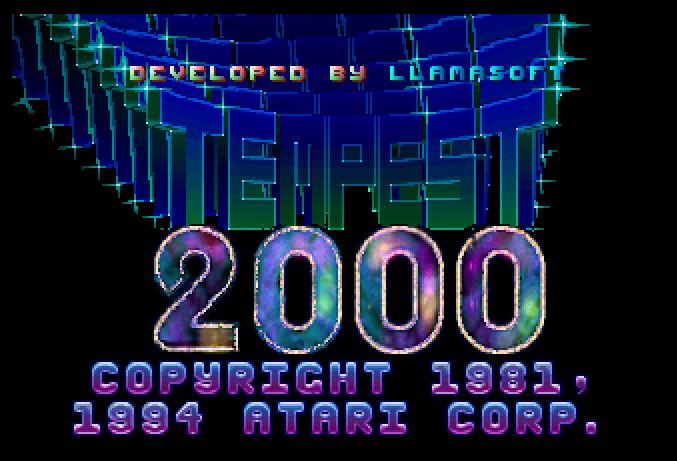
\includegraphics[width=12cm]{src/blitting/title.png}}%
    \end{adjustbox}
\caption{The title screen of Tempest 2000.}
\end{figure}

Here we find a slightly different order of business in setting up the blitting copy:

\begin{lstlisting}[escapechar=\%]
WaitBlit:
  move #4,d0         ; x position in pic5
  move #84,d1        ; y position in pic5
  move #197,d2       ; width to copy
  move #65,d3        ; height to copy
  move #92,d4        ; x pos of write to
  move #120-15,d5    ; y pos to write to
  tst pal            ; are we PAL or NTSC?
  beq mypal
  add #10,d5         ; we're NTSC so offset the y pos by 10 pixels
mypal:
  move.l #pic5,a0a   ; file 'images/beasty7.cry' again
  move.l #screen3,a1 ; destination we're copying to
  jsr CopyBlock  
\end{lstlisting}

Can you guess the piece of \icode{beasty7.cry} we're copying here? It's this:


\begin{figure}[H]
    \centering
    \begin{adjustbox}{width=12cm,center}
      \frame{
\includegraphics[width=4cm]{src/cry/beasty7.png}}%
      \hspace{0.5cm}
      
\begin{tikzpicture}
        \draw[->,line width=4pt] (0,0) to (1,0);
      \end{tikzpicture}
      \hspace{0.5cm}
      \frame{
\includegraphics[width=4cm]{src/blitting/2000.png}}%
    \end{adjustbox}
  \caption{Extracting the '2000' chunk from \icode{beasty7.cry}.}
\end{figure}

There is a little extra twiddling in our code to figure out whether the display we're on is PAL or NTSC. These were slightly conflicting standards for
analogue television display through the 1960s to the 1990s. NTSC was the standard in the US and PAL the standard in Europe. Most video games of the time 
needed to account for the slightly different dimensions each standard offered. In the case of our title screen that meant adding an extra offset of 10
pixels to the Y position of the '2000' when painting it to the screen on an NTSC set in order to ensure that it appeared correctly positioned.

Now that we've got the general idea of how to get at least some pictures on to the screen, let's take a look at how we get some text up there.

